%%%%%%%%%%%%%%%%%%%%%%%%%%%%%%%%%%%%%%%%%%%%%%%%%%%%%%%%%%%%%%%%%%%%%%%%%%%%%%%%%%%%
% Do not alter this block (unless you're familiar with LaTeX
\documentclass{article}
\usepackage[margin=1in]{geometry} 
\usepackage{amsmath, amsthm, amssymb,amsfonts, fancyhdr, color, comment, graphicx, environ}
\usepackage{xcolor}
\usepackage{mdframed}
\usepackage[shortlabels]{enumitem}
\usepackage{indentfirst}
\usepackage{hyperref}
\usepackage{algorithm2e}
\usepackage{graphicx}
\usepackage{wrapfig}
\usepackage{hyperref}
\usepackage{listings}
\lstset{ 
  language=R,                     % the language of the code
  basicstyle=\normalsize\ttfamily, % the size of the fonts that are used for the code
  numbers=left,                   % where to put the line-numbers
  numberstyle=\normalsize\color{gray},  % the style that is used for the line-numbers
  stepnumber=1,                   % the step between two line-numbers. If it is 1, each line
                                  % will be numbered
  numbersep=5pt,                  % how far the line-numbers are from the code
  backgroundcolor=\color{white},  % choose the background color. You must add \usepackage{color}
  showspaces=false,               % show spaces adding particular underscores
  showstringspaces=false,         % underline spaces within strings
  showtabs=false,                 % show tabs within strings adding particular underscores
  frame=single,                   % adds a frame around the code
  rulecolor=\color{black},        % if not set, the frame-color may be changed on line-breaks within not-black text (e.g. commens (green here))
  tabsize=2,                      % sets default tabsize to 2 spaces
  captionpos=b,                   % sets the caption-position to bottom
  breaklines=true,                % sets automatic line breaking
  breakatwhitespace=false,        % sets if automatic breaks should only happen at whitespace
  keywordstyle=\color{black},      % keyword style
  commentstyle=\color{gray},   % comment style
  stringstyle=\color{teal}      % string literal style
} 
\hypersetup{
    colorlinks=true,
    linkcolor=blue,
    filecolor=magenta,      
    urlcolor=blue,
}


\pagestyle{fancy}


\newenvironment{problem}[2][Problem]
    { \begin{mdframed}[backgroundcolor=gray!20] \textbf{#1 #2} \\}
    {  \end{mdframed}}

% Define solution environment
\newenvironment{solution}
    {\textit{Solution:}}
    {}

\renewcommand{\qed}{\quad\qedsymbol}

% prevent line break in inline mode
\binoppenalty=\maxdimen
\relpenalty=\maxdimen

%%%%%%%%%%%%%%%%%%%%%%%%%%%%%%%%%%%%%%%%%%%%%
%Fill in the appropriate information below
\lhead{Pengju Zhang}
\rhead{CSC-424} 
\chead{\textbf{Assignment 5}}
%%%%%%%%%%%%%%%%%%%%%%%%%%%%%%%%%%%%%%%%%%%%%

\begin{document}
%problem 1
\begin{problem}{1}
\textbf{[20 pts]}
Download the “kellog.dat” data file which contains data on 22 cereals from Kellog. Each cereal has 9 metric values that measure various aspects of the cereal. We are not given the meanings of these variables, but in spite of this use the data to classify the cereals:
\begin{enumerate}
	\item Read the data into a data.frame in R. Note that the data file has two extra rows, you can ignore these with the “skip=2” parameter in read.table, or you can manually delete them. Also, you will want to put the cereal names in the row.names with “row.names=1” which indicates to use the first column as the row names.
	\item Compute the distance matrix with “dist”. Just treat the ordinal and binary categorical variables as metric variables (this is actually ok here because they are either interval variables), or binary variables encoded as [0, 1].
	\item Run multidimensional scaling on the distance matrix with the “isoMDS” command from the MASS library. This computes MDS and provides a bit more and as its output, providing both an array of “\$points” to plot and a stress value. Plot the points from c) and report the stress value. How faithfully does the plot reproduce the distances in the data according to the stress value (remember the stress value from R is actually multiplied by 100 so it is a percentage)?
	\item How many clusters or groups does the data fall into? Can you identify some distinct groupings? Interpret at least two of the groupings of cereals based on their names in the data file.
	\item Run an agglomerative hierarchical clustering on the dataset and plot the result as a dendogram.
	\item At a level of 3 clusters in the dendogram, use the cutree(h, k=3) command to evaluate the clusters and then replot the MDS using these categories to color the data. Interpret the results.
	\item (Extra Credit, 3 points) Give a practical interpretation for at least one of the two dimensions in the MDS.
\end{enumerate}
\end{problem}
\begin{solution}
\href{run:./src/p1.r}{ (Problem 1 Source Code)}
\begin{enumerate}
\item\mbox{}
	\begin{lstlisting}
# output
> data = read.table("kellog.dat", skip=2, row.names=1)
> head(data)
                    V2  V3     V4     V5     V6     V7     V8  V9    V10 V11
AllBran         0.1818 0.6 0.3333 0.8125 0.6429 0.0000 0.3333 1.0 0.9677   0
AllBranFlakes   0.0000 0.6 0.0000 0.4375 1.0000 0.0667 0.0000 1.0 1.0000   0
AppleJacks      0.5455 0.2 0.0000 0.3906 0.0714 0.2667 0.9333 0.5 0.0323   0
CornFlakes      0.4545 0.2 0.0000 0.9063 0.0714 0.9333 0.1333 0.0 0.0484   0
CorPops         0.5455 0.0 0.0000 0.2813 0.0714 0.4000 0.8000 0.5 0.0000   0
CracklinOatBran 0.5455 0.4 1.0000 0.4375 0.2857 0.2000 0.4667 1.0 0.4516   0
	\end{lstlisting}
\newpage
\item\mbox{}
	\begin{lstlisting}
> kellog.x = as.matrix(data)
> kellog.dist = dist(kellog.x)
	\end{lstlisting}
\item\mbox{}
	\begin{lstlisting}
> kellog.mds = isoMDS(kellog.dist)
initial  value 19.915627 
iter   5 value 14.639105
iter  10 value 14.220989
final  value 14.179482 
converged
> kellog.mds$stress
[1] 14.17948
	\end{lstlisting}	
Stress of 14.17948 indicate approximately 14\% variance which is not a good fit.
\item\mbox{}
	\begin{figure}[h]
		\centering
		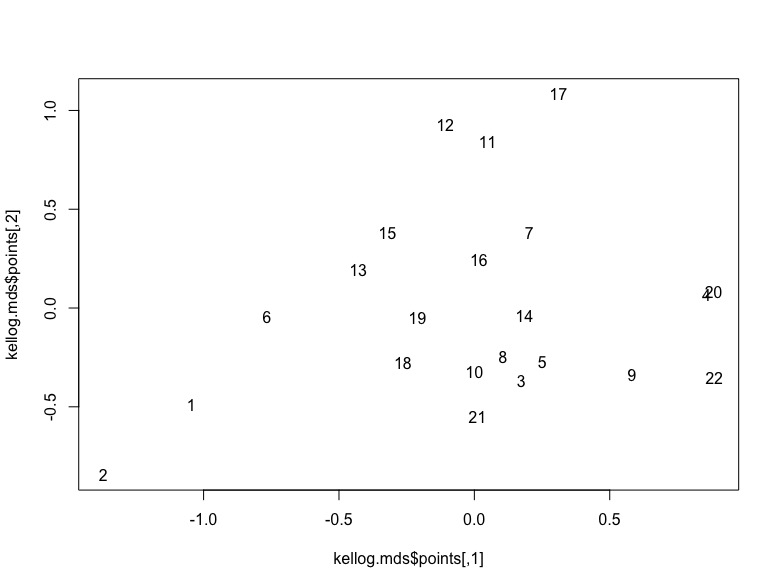
\includegraphics[width=0.7\textwidth]{Figure1_Rplot.jpeg}
		\caption{Multidimensional Scaling Plot}
	\end{figure}
From visualization perspective, there might be 3 patterns: first one contains the most condense part from -0.5 to 0.5, and other two parts are less than -0.5 and greater than 0.5.
\newpage
\item\mbox{}
	\begin{figure}[h]
		\centering
		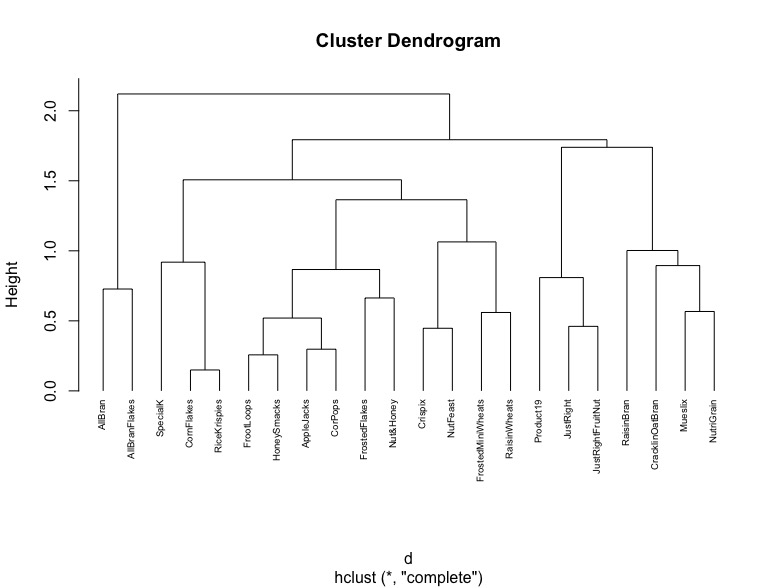
\includegraphics[width=0.5\textwidth]{Figure2_Rplot.jpeg}
		\caption{Agglomerative Hierarchical Clustering Dendrogram}
	\end{figure}
\item\mbox{}
If we using agglomerative hierarchical clustering, we can see part 2 and 3 are mostly overlap with each other, turns out a bad cluster method. Hence I switch the process from bottom-up to top-down (divisive hierarchical clustering), it gives much better result (Figure 4).
	\begin{figure}[h]
		\centering
		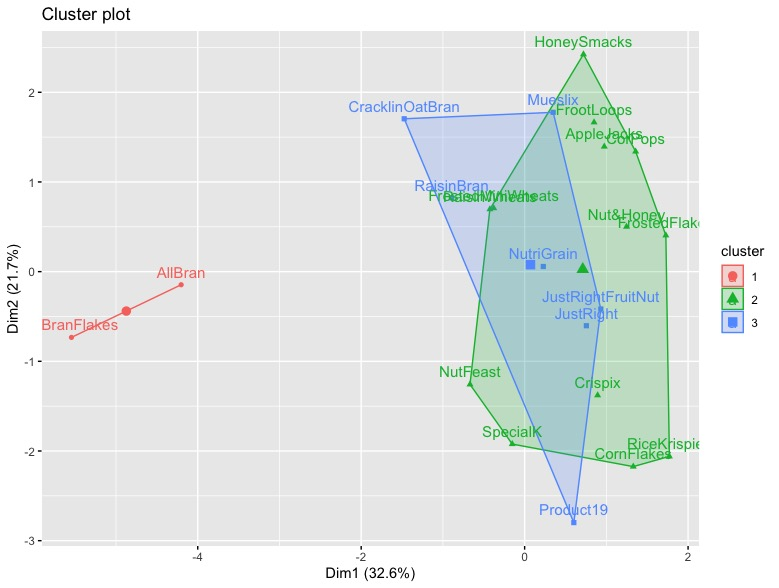
\includegraphics[width=0.7\textwidth]{Figure3a_Rplot.jpeg}
		\caption{Agglomerative Hierarchical Clustering Plot}
	\end{figure}
\newpage
	\begin{figure}[h]
		\centering
		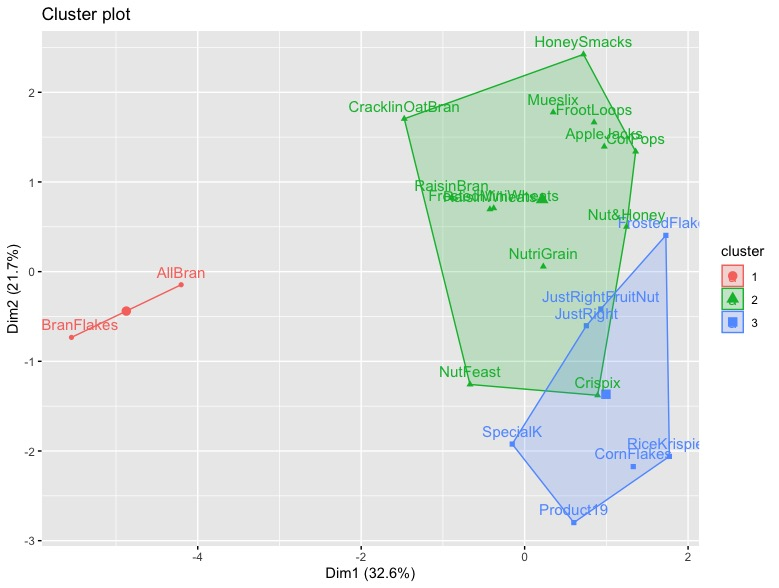
\includegraphics[width=0.7\textwidth]{Figure3b_Rplot.jpeg}
		\caption{Divisive Hierarchical Clustering Plot}
	\end{figure}
\end{enumerate}
\end{solution}
\newpage
%problem 2
\begin{problem}{2}
\textbf{[10 pts]}
Perform a canonical correlation analysis, describing the relationships between the soil and water variables using the data1 found in data\_marsh\_cleaned.csv.
\begin{enumerate}
	\item Answer the following questions regarding the canonical correlations. (Note that a, b and c can all be done directly from the output of canonical correlation)
	\begin{enumerate}
		\item Test the null hypothesis that the canonical correlations are all equal to zero. Give your test statistic, d.f., and p-value.
		\item Test the null hypothesis that the second and third canonical correlations equal zero. Give your test statistic, d.f., and p-value.
		\item Test the null hypothesis that the third canonical correlation equals zero. Give your test statistic, d.f., and p-value.
		\item Present the three canonical correlations and list any conclusions that you can draw.
	\end{enumerate}
	Answer the following questions regarding the canonical variates.
	\begin{enumerate}
		\item Give the formulae for the first canonical variate for the soil and water variables.
		\item Give the correlations between the significant canonical variates for soils and the soil variables, and the correlations between the significant canonical variates for water and the water variables and use these to interpret the variates (do this as best as you can. Even with a lack of domain knowledge you should be able to describe the relationship in more general terms given the variables involved and the correlations.)
	\end{enumerate}
\end{enumerate}
\end{problem}
\begin{solution}
\begin{enumerate}
	\item\mbox{}
		\begin{lstlisting}
> round(wilksSoil, 2)
# output
     WilksL    F df1    df2    p
[1,]   0.70 4.05  15 433.81 0.00
[2,]   0.82 4.18   8 316.00 0.00
[3,]   0.93 4.09   3 159.00 0.01
	\end{lstlisting}
The first variance and all other variances followed has information, so we want to include the first variance. Second one has p-value of 0 which can reject the null hypothesis, so it is sufficient to capture the correlation, same as third one, it has p-value of 0.01 which is significantly different from zero as well. Thus we want include all three variances.
\newpage
	\item\mbox{}
		\begin{lstlisting}
> round(-loadingsSoil$corr.X.xscores, 2)
          [,1]  [,2]  [,3]
MEHGSWB   0.21  0.54 -0.06
TURB      0.12  0.03 -0.50
DOCSWD    0.89  0.39 -0.02
SRPRSWFB  0.17 -0.58  0.64
THGFSFC  -0.49  0.62  0.53
> round(-loadingsSoil$corr.Y.yscores, 2)
        [,1]  [,2]  [,3]
THGSDFC 0.01  0.88  0.47
TCSDFB  0.64  0.77 -0.04
TPRSDFB 0.71 -0.15  0.68
	\end{lstlisting}
In terms of evaluate the overall level of correlation, we can see that it is improved by overall improvement in all of the attributes except THGFSFC. If we are concentrating on overall performance, we want to focus on DOCSWD since it has much higher correlation than others. For second column, it shows that MEHGSWB and THGFSFC have the most impact on THGSDFC and TCSDFB.
\end{enumerate}
\end{solution}
\end{document}